\section{The Bundle-Trading-Market Framework}
\label{sec:btm}
To start with, we explained in section \ref{sec:lem} that LEM enable the trading 
of locally generated energy through a market platform, market mechanism and market access for 
small-scale prosumer and consumer. 
In addition, we presented in section \ref{sec:components_of_local_energy_markets} 
a market mechanism as one of seven core components for the efficient operation of blockchain-based
LEM.

On account of that, this chapter covers and explains in detail the applied market mechanism in the BLEMS. 

As already briefly introduced in the sections \ref{sec:research_motivation} 
and \ref{sec:Distributed Resource Optimization}, the applied market mechanism is implemented 
through the developed market-based optimization algorithm, which is also called the 
BTM. 
In the proposed framework by \shortciteA{guo2012computational}, independent, self-interested
agents trading bundled resources in a double-auction market, which run by a dealer. 
In this case, the dealer replaces the central authority and agents represent distributed
entities. Generally, the BTM consists of a master problem that solves the \textit{market matching problem (MMP)}, which is managed by the dealer
and subproblems that solve the bundle-determination problem of the agents.
Further, the solution process is an iteration between the MMP and the 
the bundle-determination problems \shortcite{guo2007market}.
Considering, the BTM constitutes a market-based decomposition method 
for decomposable linear systems,
which can be easily implemented to support real-time optimization 
of distributed systems \shortcite{guo2007market}.
Likewise, the central problem of the BTM can be interpreted as the welfare optimization of all participants in LEM. 
The dealer, which runs the double auction market, maximizes the welfare through allowing 
agents to trade their preferable bundles of energy.
Therefore, the BTM is a suitable market mechanism for the concept of LEM.

\subsection{Problem Overview}
\label{sec:btm_problem_overview}
This subsection will give an introductory description to the overall problem. 
With reference to \shortciteA{guo2012computational}, we consider a distributed 
system with $k$ independent agents.
In addition, we have a central problem and individual problems of the $k$ individual agents, which both can be expressed as the 
LPs shown the in equations (\ref{eq:central_problem}) and (\ref{eq:agent_problem}). 
Besides, the BTM presented by \shortciteA{guo2007market} requires 
a nondegenerate central problem with a bounded solution. In contrast to discrete markets where 
only integer number of units can be traded, the proposed framework facilitates continuous trade amounts. 

\paragraph*{Central Problem}
\begin{equation}
\label{eq:central_problem}
 \begin{array}{ll@{}ll}
 Z(c) = \underset{x_{j} \geq 0}{\text{min}} & \displaystyle\sum\limits_{j=1}^{k} d^{T}_{j}x_{j} &\\
 \text{s.t.}& \displaystyle N_{j}x_{j} \leq n_{j}, &&j=1 ,..., k \\
 & \displaystyle\sum\limits_{j=1}^{k} C_{j}x_{j} \leq c
 \end{array}
\end{equation}

\paragraph*{Agent Problem ($j=1, ..., k$)}
\begin{equation}
    \label{eq:agent_problem}
 \begin{array}{ll@{}ll}
 z_{j}(c_{j}) = \underset{x_{j} \geq 0}{\text{min}} & \displaystyle d^{T}_{j}x_{j} &\\
 \text{s.t.}& \displaystyle N_{j}x_{j} \leq n_{j}, &&\\
 & \displaystyle C_{j}x_{j} \leq c_{j}
 \end{array}
\end{equation}

In the table below, the applied variables in the stated equations are described:


\begin{longtable}{c|l}
    \caption{Applied Variables in BTM Framework}
    \label{table:applied_variables_in_btm}
    \\
    \textbf{Variable} & \textbf{Description} \\
	\hline
    $d_{j} \in R^{b_{j}}$ & vector of agents $j's$ costs \\
    $x_{j} \in R^{b_{j}}$ & decision variables controlled by agent j \\
    $N_{j} \in R^{a_{j} \times b_{j}}$ & activity matrix \\
    $C_{j} \in R^{m \times b_{j}}$ & activity matrix \\
    $n_{j} \in R^{a_{j}}$ & capacity vector of agent $j's$ independent resources \\
    $c_{j} \in R^{m}$ & agent $j's$ vector of shared resources \\
\end{longtable} 

Further, the overall objective of the central problem is to minimize the operating costs of the overall system. The minimization of the central problem
has to be implemented in consideration of the operational constraints 
(first set of constraints) and the total shared resources capacity constraints (second set of constraints) of each individual agent. 
Nevertheless, it is assumed that the optimal solution to the central problem cannot be directly calculated, due to the lack of access to all relevant
information to make the decisions ($d_{j}, n_{j}, c_{j}, N_{j}, C_{j},$ for $j=1, ..., k$). 
Additionally, \shortciteA{guo2007market} stated that, for an allocation of 
$c_{j}, j=1, ..., k$, such that $C_{j}x_{j}^{*} \leq c_{j}, \sum\limits_{j=1}^{k} C_{j}$, 
solving the agents’ problems is equivalent to solving the central problem.

Hence, a market-based resource allocation mechanism to coordinate decentralized
decision making from agents is used by the BTM. 
For any initially given $c_{j}, j=1, ..., k$, these mechanism enables an indirectly
acquisition of an optimal solution to the central problem through a direct, iterative and
wealth-improving bidding process among the self-interested agents. 


\subsection{Market Environment}
Generally, a dealer and $k$ independent agents constitute the whole market economy. 
Each of the agents has the opportunity to trade the shared resources $c_{j}$ 
in a double auction market, which is operated by the dealer. Moreover, each agent only has a local perspective 
and knowledge, that is to say, they don't know anything about the production decisions of the others. 
Further, the market prices to match the trades will be determined and published by the dealer.
Subsequently, the roles of the market participants are described
and the market operations like the agent bidding, market matching, 
and settlement are outlined. Finally, a summary of the market-based algorithm is presented. 

\subsubsection{Agent Bidding}
\label{sec:agent_bidding}
Firstly, the initialization takes place, which means that each of the $j=1, ..., k$ agents receive an initial
endowment of the $m$ shared resources $c_{j}$ , and a cash endowment $e_{j}$.
The wealth of an agent at any point is defined as $e_{j} - z_{j}(c_{j})$ \shortcite{guo2007market}.
The agents have the opportunity to buy additional resources or to sell some of their own resources to lower their operating costs. 
Therefore, each agent knows the current market prices $p \in R^{m}$ for the shared resources, 
which are published by the dealer after each auction round. Further, for trading the shared resources in the market, 
a bundle referring to \shortciteA{guo2012computational} is defined:

\paragraph*{Bundle} A bundle $w \in R^{m}$ is an $m$-dimensional vector of shared resources. 
Each of the $m$ elements corresponds to an amount of one specific shared resource. 
A negative sign of an element signifies a sell amount, 
and contrary, a positive sign signifies a buy amount. \newline


An \textit{improving bundle set} concerning to lower operating costs is defined as the following:

\paragraph*{Improving Bundle Set}
\begin{equation}
 \begin{array}{ll@{}ll}
 W_{j}(c_{j}|p) = \{w: \exists x_{j} \geq 0 \ni d_{j}^{T}x_{j} + p^{T}w \leq z_{j}(c_{j}), \\
 N_{j}x_{j} \leq n_{j}, C_{j}x_{j} \leq c_{j}+w \}
 \end{array}
\end{equation}

To remember that $z_{j}(c_{j})$ is the optimal value of the agent $j's$ problem depending on the amount of the shared resources $c_{j}$. 
That means, an agent looking for bundles that satisfy 
$d_{j}^{T}x_{j} + p^{T}w \leq z_{j}(c_{j})$. If 
$p^{T}w \geq 0$, the term $p^{T}w$ is interpreted as the payment to receive the bundle $w$.
For the opposite, if $p^{T}w \leq 0$, the term $p^{T}w$ constitutes the revenue for selling the bundle $w$.


Accordingly, a rational agent will choose an improving bundle for trading, 
which leaves his wealth on the same level or better off. 
In addition, the basic market mechanism of \shortciteA{guo2007market} assumes no 
strategic actions in the bundle selection and pricing. However, strategic actions 
can be relaxed and \shortciteA{guo2012computational} also incorporate strategic factors
in their extended BTM. 
Nevertheless, the applied market mechanism in the BLEMS implemented nonstrategic bidding, wherefore an agents bundle selection 
can be defined as the following \textit{Bundle Determination Problem (BDP):}

\paragraph*{Bundle Determination Problem}
\begin{equation}
 \begin{array}{ll@{}ll}
 \underset{x_{j} \geq 0, w}{\text{min}} & \displaystyle d^{T}_{j}x_{j} + p^{T}w &\\
 \text{s.t.}& \displaystyle N_{j}x_{j} \leq n_{j}, &&\\
 & \displaystyle C_{j}x_{j} \leq c_{j}+w
 \end{array}
\end{equation}

According to \shortciteA{guo2007market}, the BDP have either 
a bounded, or an unbounded solution. A bounded solution is called \textit{limited bundle} 
$w \in R^{m}$, whereby an unbounded solution is called \textit{unlimited bundle}
$u \in R^{m}$.

Furthermore, each agent needs to determine a limit price, which indicates
the maximum an agent is willing to pay for the bundle. 
As already explained above, nonstrategic pricing is implemented. 
Therefore, an agent will always submits a limit price equal to the valuation of the bundle. That is to say, $l(w) = v(w)$.

For a limited bundle $w$, the value $v(w)$ is defined as:

\begin{equation*}
 \begin{array}{ll@{}ll}
 z_{j}(c_{j}) - z_{j}(c_{j} + w) = z_{j}(c_{j}) - d_{j}^{T}x_{j}.
 \end{array}
\end{equation*}

Whereas for a unlimited bundle $u$, the value $v(u)$ describes the 
unit-incremental value that $u$ contributes to the objective change. It is defined
as:

\begin{equation*}
 \begin{array}{ll@{}ll}
 -d_{j}^{T}\hat{x_{j}}.
 \end{array}
\end{equation*}

Potentially, an agent has multiple optimal solutions in his bundle-determination problem. Hence, it is allowed to submit more than
one bundle at a time. 

Finally, old orders and bids of prior rounds without any trades will be treated 
as open orders and bids, because the valuation of an agent for a bundle is
independent of the market price $p$.
It only depends on the respective resource level $c_{j}$. 

\subsubsection{Market Matching Mechanism}
\label{sec:market_clearing_mechanism}
The BLEMS applied a synchronous call market where the market prices $p$ are announced periodically by the market dealer. 
However, the synchronous requirement can be relaxed through the 
asynchronous market trading environment introduced by \shortciteA{guo2012computational} . 

The dealer trades on its own account and has also an 
initial cash endowment $e_{0}$ and resource endowment $c_{0}$.
The sum of all resource endowments needs to fulfill the following equation:

\begin{equation*}
 \begin{array}{ll@{}ll}
 \sum\limits_{j=1}^{k} c_{j} + c_{0} \leq c
 \end{array}
\end{equation*}

Next, agents submit sealed bids to the dealer. The dealer maintains an individual order book for each agent. 
Each individual order book contains two different order sets. On the one hand, the set for limited orders $I_{j}$,
on the other hand, the set for unlimited orders $H_{j}$.
If an agent submits orders and no trade is executed, the orders are collected and 
accumulated for the respective agent. Otherwise, any trade from an agent will clear the respective order book,
as it cannot be safely assumed that an old bundle still improves the agents LP given its new resource endowment.
To determine the maximal trade surplus the dealer solves the following MMP:

\paragraph*{Market Matching Problem}

\begin{equation}
\label{eq:mmp}
 \begin{array}{ll@{}ll}
 \underset{y_{j}^{i} \geq 0, t_{j}^{h} \geq 0 }{\text{max}} & 
 \sum\limits_{j=1}^{k}
 \left(\sum\limits_{i \in I_{j}}^{} l_{j}(w_{j}^{i})y_{j}^{i} + 
 \sum\limits_{h \in H_{j}}^{} l_{j}(u_{j}^{h})t_{j}^{h} \right) &\\
 \text{s.t.}
 & \sum\limits_{j=1}^{k}
 \left(\sum\limits_{i \in I_{j}}^{} w_{j}^{i}y_{j}^{i} + 
 \sum\limits_{h \in H_{j}}^{} u_{j}^{h}t_{j}^{h} \right) \leq c_{0} \\
 & \sum\limits_{j=1}^{k} y_{j}^{i} \leq 1, \quad j=1 ,..., k
 \end{array}
\end{equation}

Considering the first set of constraints, if $c_{0} = 0$, it is required that any buy amounts be met by sell amounts. 
On the opposite, if $c_{0} \neq 0$, the dealer supplies additional resources from the inventory
to meet buys. 

The second set of constraints indicate that the market handles limited and unlimited bundles differently. 
The trades of unlimited bundles in $H_{j}$ are unrestricted, whereas limited bundles in $I_{j}$
are restricted. In that case, limited trades are restricted to be convex combinations of bundles in $I_{j}$.

Besides, the MMP always has a solution, because setting all variables to zero 
is always a feasible solution. As described by \shortciteA{guo2007market}, the market closes when no trade takes place 
and the market prices remain unchanged. Finally, if the MMP has a nonzero solution for
 $y_{j}^{i^{*}}$, for $i \in I_{j}$ and $t_{j}^{h^{*}}$, for $h \in H_{j}$, then agent $j$ will have traded the following:

 \begin{equation*}
 \begin{array}{ll@{}ll}
 w_{j}^{*} = 
 \sum\limits_{i \in I_{j}}^{} w_{j}^{i}y_{j}^{i^{*}} + 
 \sum\limits_{h \in H_{j}}^{} u_{j}^{h}t_{j}^{h^{*}}.
 \end{array}
\end{equation*}

The market clearing prices $p \in R^{m}$ are derived from the dual values of the first set of constraints in the MMP
(to remember, the concept of duality is explained in section \ref{sec:duality_theory}).
Consequently, the settlement price for an agent who have traded resources are the following:

\begin{equation*}
 \begin{array}{ll@{}ll}
 p^{T} w_{j}^{*}.
 \end{array}
\end{equation*}

In the following, the whole settlement process is summarized and the calculation of the new values of agent $j$ and the dealer 
is outlined:

\paragraph*{Agent $j$:}
\begin{equation*}
 \begin{array}{ll@{}ll}
 c_{j} \leftarrow c_{j} + w_{j}^{*} \\
 e_{j} \leftarrow e_{j} + p^{T} w_{j}^{*} \\
 \end{array}
\end{equation*}

\paragraph*{Dealer:}
\begin{equation*}
 \begin{array}{ll@{}ll}
 c_{0} \leftarrow c_{0} + \sum\limits_{j=1}^{k} w_{j}^{*} \\
 e_{0} \leftarrow e_{0} + \sum\limits_{j=1}^{k} p^{T} w_{j}^{*} \\
 \end{array}
\end{equation*}

\subsubsection{Summary of BTM}
\label{sec:summary_of_btm}
This subsection gives a summarized overview of the BTM, which 
is based on the equations (\ref{eq:central_problem})-(\ref{eq:mmp}) and 
present a belonging flowchart in Figure \ref{figure:btm_flowchart}.

\begin{description}
 \item[Input] \hfill \\
 Initial allocations: $e_{j}, c_{j}$, for $j=1,...,k$, and \\
 initial market prices: $p \geq 0$.
 \item[Output] \hfill \\
 Optimal solutions $x_{j^{*}}$ to the central problem, \\
 optimal allocations $c_{j^{*}}$, for $j=1,...,k$, and \\
 optimal market prices $p^{*}$.
 \item[Step 0] \hfill \\
 Set $I_{j} = \emptyset, H_{j} = \emptyset$, for $j=1,...,k$, and \\
 the last market-price vector $\pi = 0$.
 \item[Step 1] \hfill \\
 The dealer saves the current market prices $\pi \leftarrow p$. Each agent solves his 
 BDP and adds new limited bundle orders to $I_{j}$ and 
 unlimited bundle orders to $H_{j}$.
 \item[Step 2] \hfill \\
 The dealer solves the MMP ($w_{j}^{*}$ represents a matched bundle for agent $j$). 
 \item[Step 3] \hfill \\
 If no nonzero solution exists, this step will be skipped and continued with \textit{Step 4}.
 If a nonzero solution to the MMP exists and the trades include items from at least one agent and the dealer, the settlement takes place. 
 The dealer publishes the shadow prices $p$ as the new market prices.
 The new allocations are calculated as follows:
 $c_{j} \leftarrow c_{j} + w_{j}^{*}$, for $j=1,...,k$ and $c_{0} \leftarrow c_{0} + \sum\limits_{j=1}^{k} w_{j}^{*}$.
 Further, the new endowments are calculated as follows:
 $e_{j} \leftarrow e_{j} + p^{T} w_{j}^{*}$ for $j=1,...,k$ and $e_{0} \leftarrow e_{0} + \sum\limits_{j=1}^{k} p^{T} w_{j}^{*}$.
 Reset $I_{j} = \emptyset$ and $H_{j} = \emptyset$ for each agent $j$ with $w_{j}^{*} \neq 0$.
 Now, go to \textit{Step 1}. 
 \item[Step 4] \hfill \\
 The dual values of the clearing constraints from the MMP form the new market prices $p$. 
 If the new market prices $p \neq \pi$ , go to \textit{Step 1}, otherwise, stop.
\end{description}

\begin{figure}[htbp]
        \centering
        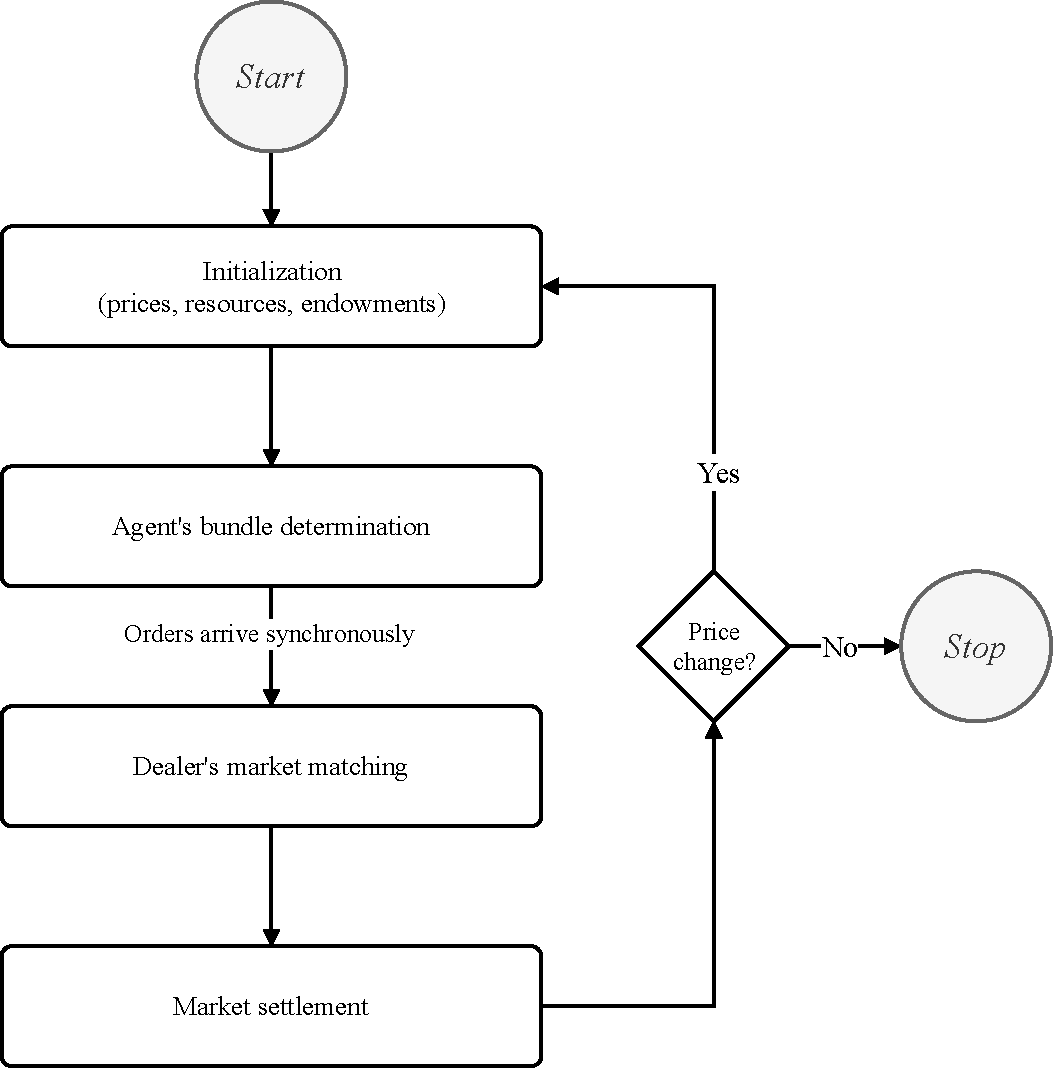
\includegraphics[width=0.59\linewidth]{./figures/btm_flowchart.pdf}
        \caption{Flowchart of BTM, inspired by \protect\shortciteA{guo2012computational}}
        \label{figure:btm_flowchart}
\end{figure}


\clearpage